\documentclass{article} % For LaTeX2e
\usepackage{nips13submit_e,times}
\usepackage{hyperref}
\usepackage{url}
\usepackage{graphicx}
\usepackage{caption}
\usepackage{cite}


\title{An Exploration of Face Space}


\author{
Durmus U. Karatay \\
Department of Physics \\
University of Washington \\
\texttt{ukaratay@uw.edu}
\And
Mathias Smith \\ 
Department of Physics \\
University of Washington \\
\texttt{mwsmith2@uw.edu}
}

\nipsfinalcopy
\begin{document}

\maketitle

\begin{abstract}
The project aims to utilize algorithms which can distinguish features in a set of images.  We employ Principal Component Analysis (PCA) and Linear Discriminant Analysis (LDA).  PCA allows us to identify features based on image similarities, and LDA helps distinguish between features.  
\end{abstract}

\section{Introduction}

In this work we explore a well known approach for facial recognition using PCA and LDA.  PCA treats the system as 2-dimensional and projects face images into a face-space that has the information of the variation among the training images. The basis of this face-space is referred to as eigenfaces.  We try to identify different sets of image features by calculating the projections of eigenfaces onto the images.  However, PCA cannot differentiate well between 3-dimensional rotations and different lighting conditions.  These shortcomings limit the usefulness of PCA in facial recognition.

LDA can compensate for the shortcomings of PCA if they are used in conjunction.  LDA produces well separated classes in a low dimensional face-space, even under the conditions discussed above.  We aim to use PCA for recognition of individuals and PCA together with LDA for recognition of facial features.

The dataset that we used for this experiment can be downloaded online\footnote{\url{http://www.cs.cmu.edu/afs/cs.cmu.edu/project/theo-8/faceimages/faces/}}.  The data consists of about 2000 images of 20 different individuals with three different characteristic features: orientation, facial expression, inclusion of sunglasses.  We randomly divide the dataset into a test set and training set, training set being 65\% of the data.

\section{Methods}

\subsection{PCA}

Given $N$ images, there are $K$ ($\leq N$) most significant eigenfaces to approximate a face. All images are $W \times H$ matrices which are rearranged into $W H \times 1$ column vectors referred to as $\Gamma_i$.  We calculate the average face as

\[
	\Psi = \frac{1}{N} \sum_{i = 1}^{N} \Gamma_i.
\]

We center each face by subtracting off $\Psi$, then we construct the our image matrix, $\mathbf{A}$.

\[ 
	\Phi_i = \Gamma_i - \Psi.
\]
\[
	\mathbf{A} = \left[ \Phi_1, \Phi_2, ..., \Phi_N \right].
\]

Since it is computationally expensive to calculate the eigenvectors of such a large matrix, we employ the method described in the original work of Turk et al \cite{tur91}.  

\[
	\mathbf{C} = \mathbf{A} \mathbf{A}^T.
\]

We obtain the eigenvectors of $\mathbf{C}$, $u_i$, by first calculating the eigenvectors of $\mathbf{A^T A}$, namely $v_i$.  

\[
	u_i = \mathbf{A} v_i.
\]

We need to select the most significant $K$ eigenvectors by looking at the eigenvalues.  The variance, $\sigma$ can be used to determine $K$ by selecting a threshold on the fractional variance, $F(\sigma, K)$.

\[
	\sigma = \sum_{i=1}^{N} \lambda_i, \\
\]
\[
	F(\sigma, K) = \frac{\sum_{i=1}^{K} \lambda_i}{\sigma}.
\]

The images in the training set are characterized by calculating the projection of the first $K$ eigenvectors onto the image:

\[
	\omega_{ij} = u_j^T \Phi_i.
\]

For recognition of an unknown image, we center the image by subtracting $\Psi$ and calculate the weight for each eigenface.  With these weights we can test against our training set weights to determine which subject it is.  So far in our experiments, we have used the Euclidean distance metric as our classifier. Nonetheless, we will explore Gaussian mixture models, support vector machines, and nearest neighbor method in further studies.

We implemented the PCA algorithm in Python\footnote{2.7.5}. In our dataset we have three different resolutions ($120\times128$, $60\times64$, and $30\times32$) for the same set of images.  We test our implementation on a subset of regularly oriented faces without any accessories for each of the resolutions over fractional variances ranging from $0.5 - 1.0$.

\begin{minipage}{0.5\textwidth}
	\centering
	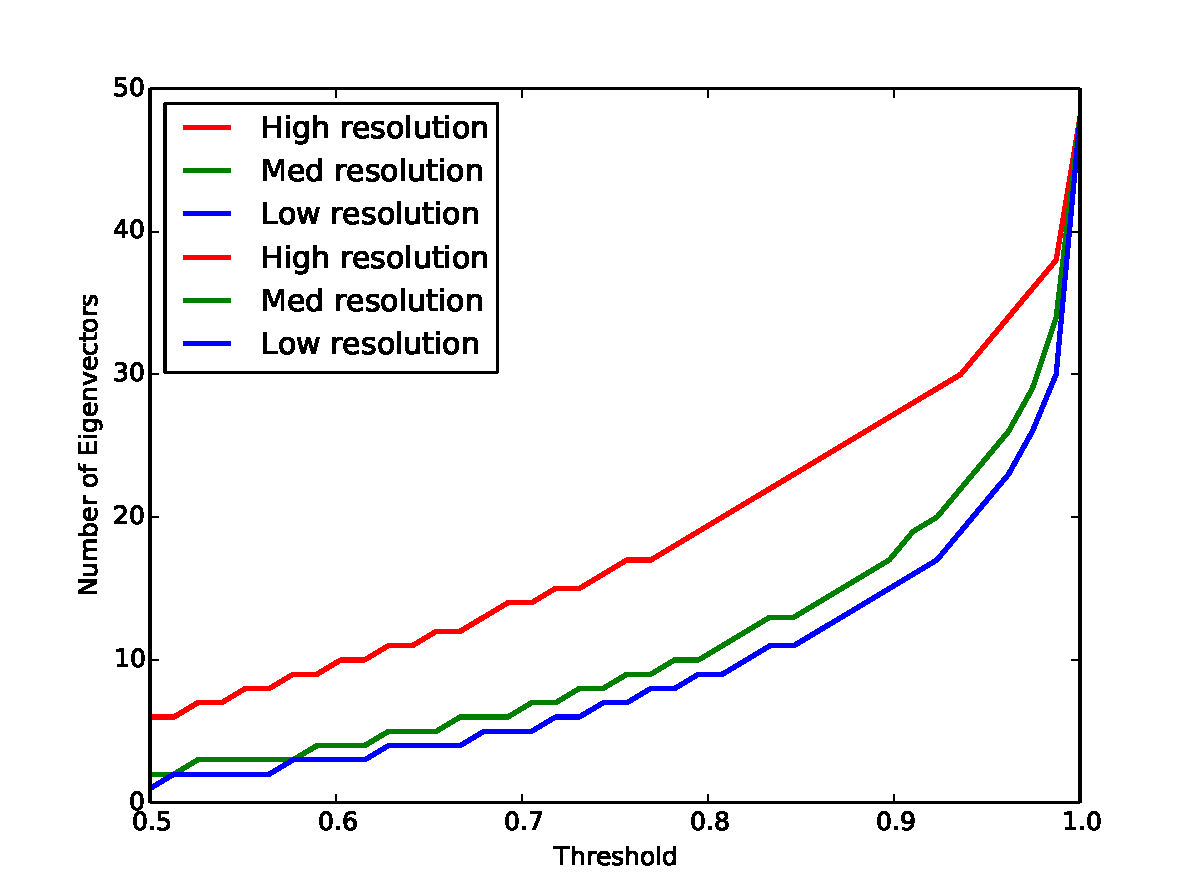
\includegraphics[width=1.0\linewidth]{fig/neig.pdf}
	\captionof{figure}{The number of eigenvectors $K$ for different threshold values.}
	\label{fig:neig}
\end{minipage}
\hfill
\begin{minipage}{0.5\textwidth}
	\centering
	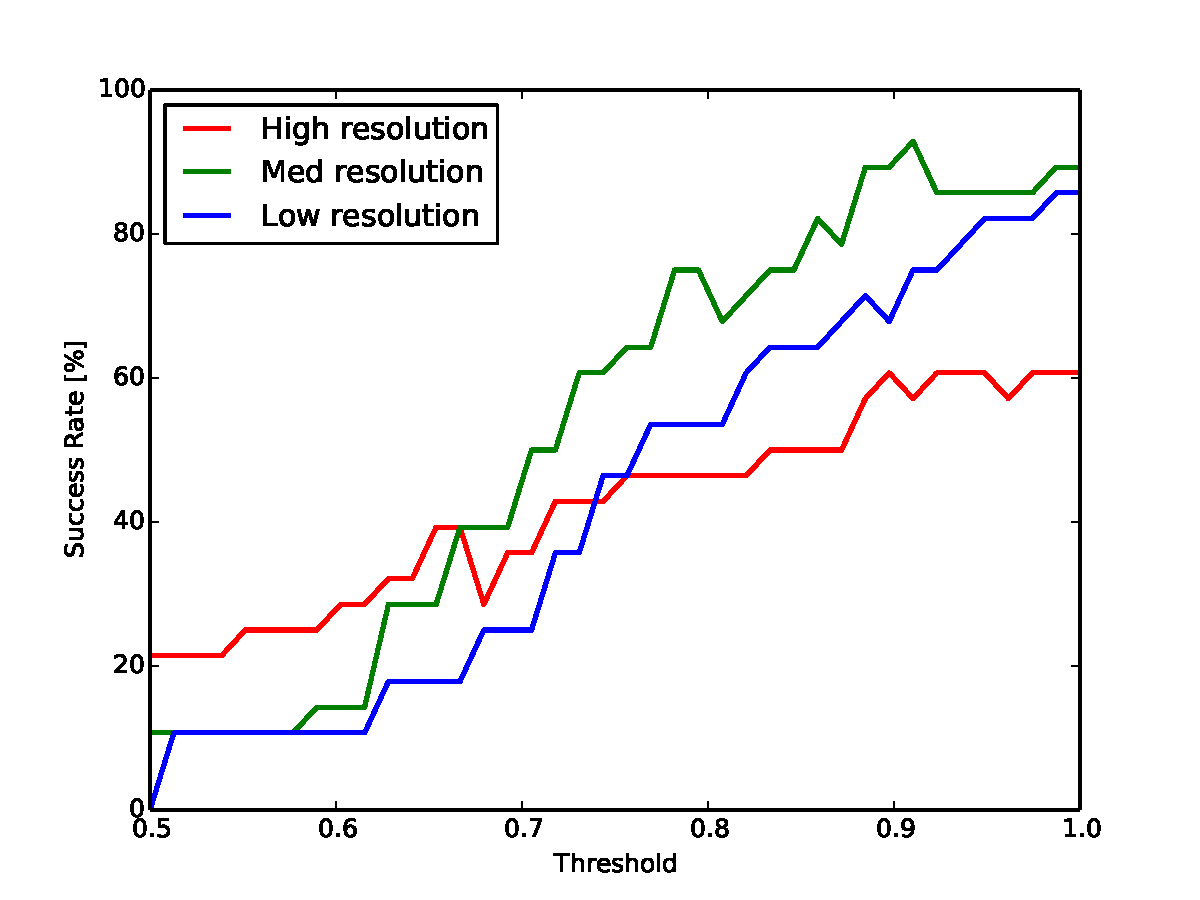
\includegraphics[width=1.0\linewidth]{fig/rate.pdf}
	\captionof{figure}{The success rate for different threshold values.}
	\label{fig:rate}
\end{minipage}

The highest success rate, 92.86\%, occurs for the medium resolution when the fractional variance threshold was set to 0.91.  For these parameters $K$ is 19.

For the low resolution images, using more eigenfaces increases the success rate; however, it is computationally restrictive to use too large a number eigenfaces.  High resolution perform better for low fractional variances thresholds, but tend to overfit as more eigenfaces are incorporated.  

\begin{figure}[h]
	\centering
	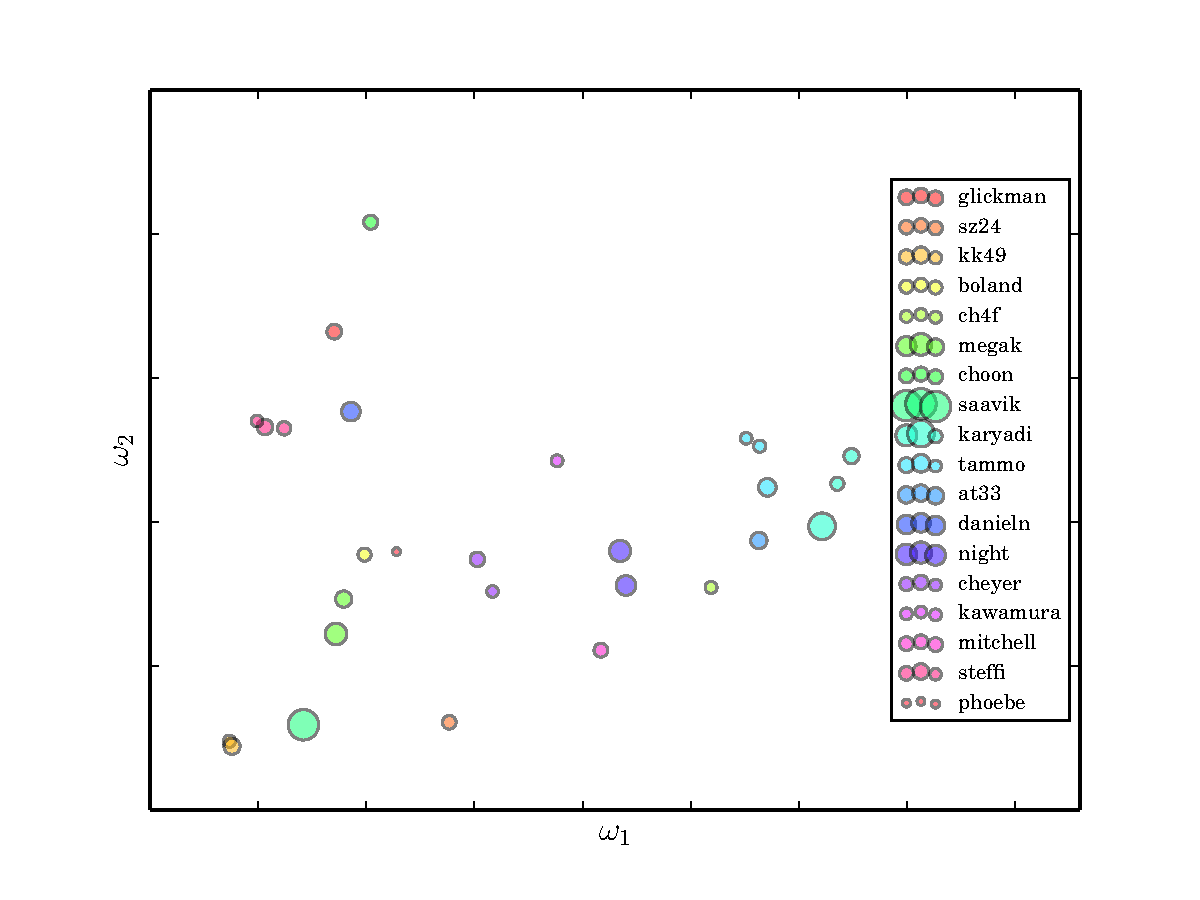
\includegraphics[width=1.0\linewidth]{fig/scatter_by_name.pdf}
	\caption{A scatter plot of test results for the optimal parameter values.  The axes are the weights for the eigenfaces corresponding to the two largest eigenvalues, the size of each marker is proportional to the Euclidean distance from training data, and the each corresponds to a person in the dataset.}
	\label{fig:scatter}
\end{figure}

Figure \ref{fig:scatter} clearly shows the clustering of faces in the test data.  Each test image is identified based on minimizing the Euclidean distance from samples available in the training data.  The minimum corresponds to an individual and the test image is classified as that individual.  The size of the marker is proportional to the total Euclidean distance form the trained characteric weights.  

\subsection{LDA}

As was stated before, PCA does not work well under different lighting conditions and 3-dimensional rotations.  Belhumeur et al developed the Fisherfaces Method which uses Fisher Linear Discriminant Analysis\cite{bel97}.  Their LDA method performs better and has lower error rates than the eigenface technique on the same set of images when the lighting and position of the face are varied.  We will explore the use of LDA in conjunction with PCA in the coming weeks.

\section{Conclusion}

In this part of the project we implemented PCA and explored the effect of thresholds and resolutions on the success rate of facial recognition.  We achieved a success rate close to those reported in literature.  Future tests will use more complex datasets and LDA methods to enhance PCA.

\newpage
\bibliography{rmf}{}
\bibliographystyle{unsrt}

\end{document}